%!TEX root = /Users/Daniel/Documents/Imperial/project/tevatron-higgs/report/report.tex

The Monte Carlo simulation of the events used in the training and evaluation of the neural networks is beyond the scope of this project, so will only be briefly summarised here. Signal $\phi b \rightarrow b\bar{b}b $ events were simulated using the PYTHIA event generator \cite{sjostrand2006pythia} to leading order, with a mass hypothesis  of $M_H = 110 \mathrm{GeV/c^2}$ and then corrected to next-to-leading order with MCFM \cite{campbell2010mcfm}. 
The background multijet events were generated using ALPGEN \cite{mangano2003alpgen}. The simulated events were then passed through a model of the D$\emptyset$ detector \cite{brun1993geant}.
Finally various preprocessing cuts were applied to the data excluding unlikely signal events, giving a final total of 53,960 events.


\begin{figure}[htbp]
	\centering
		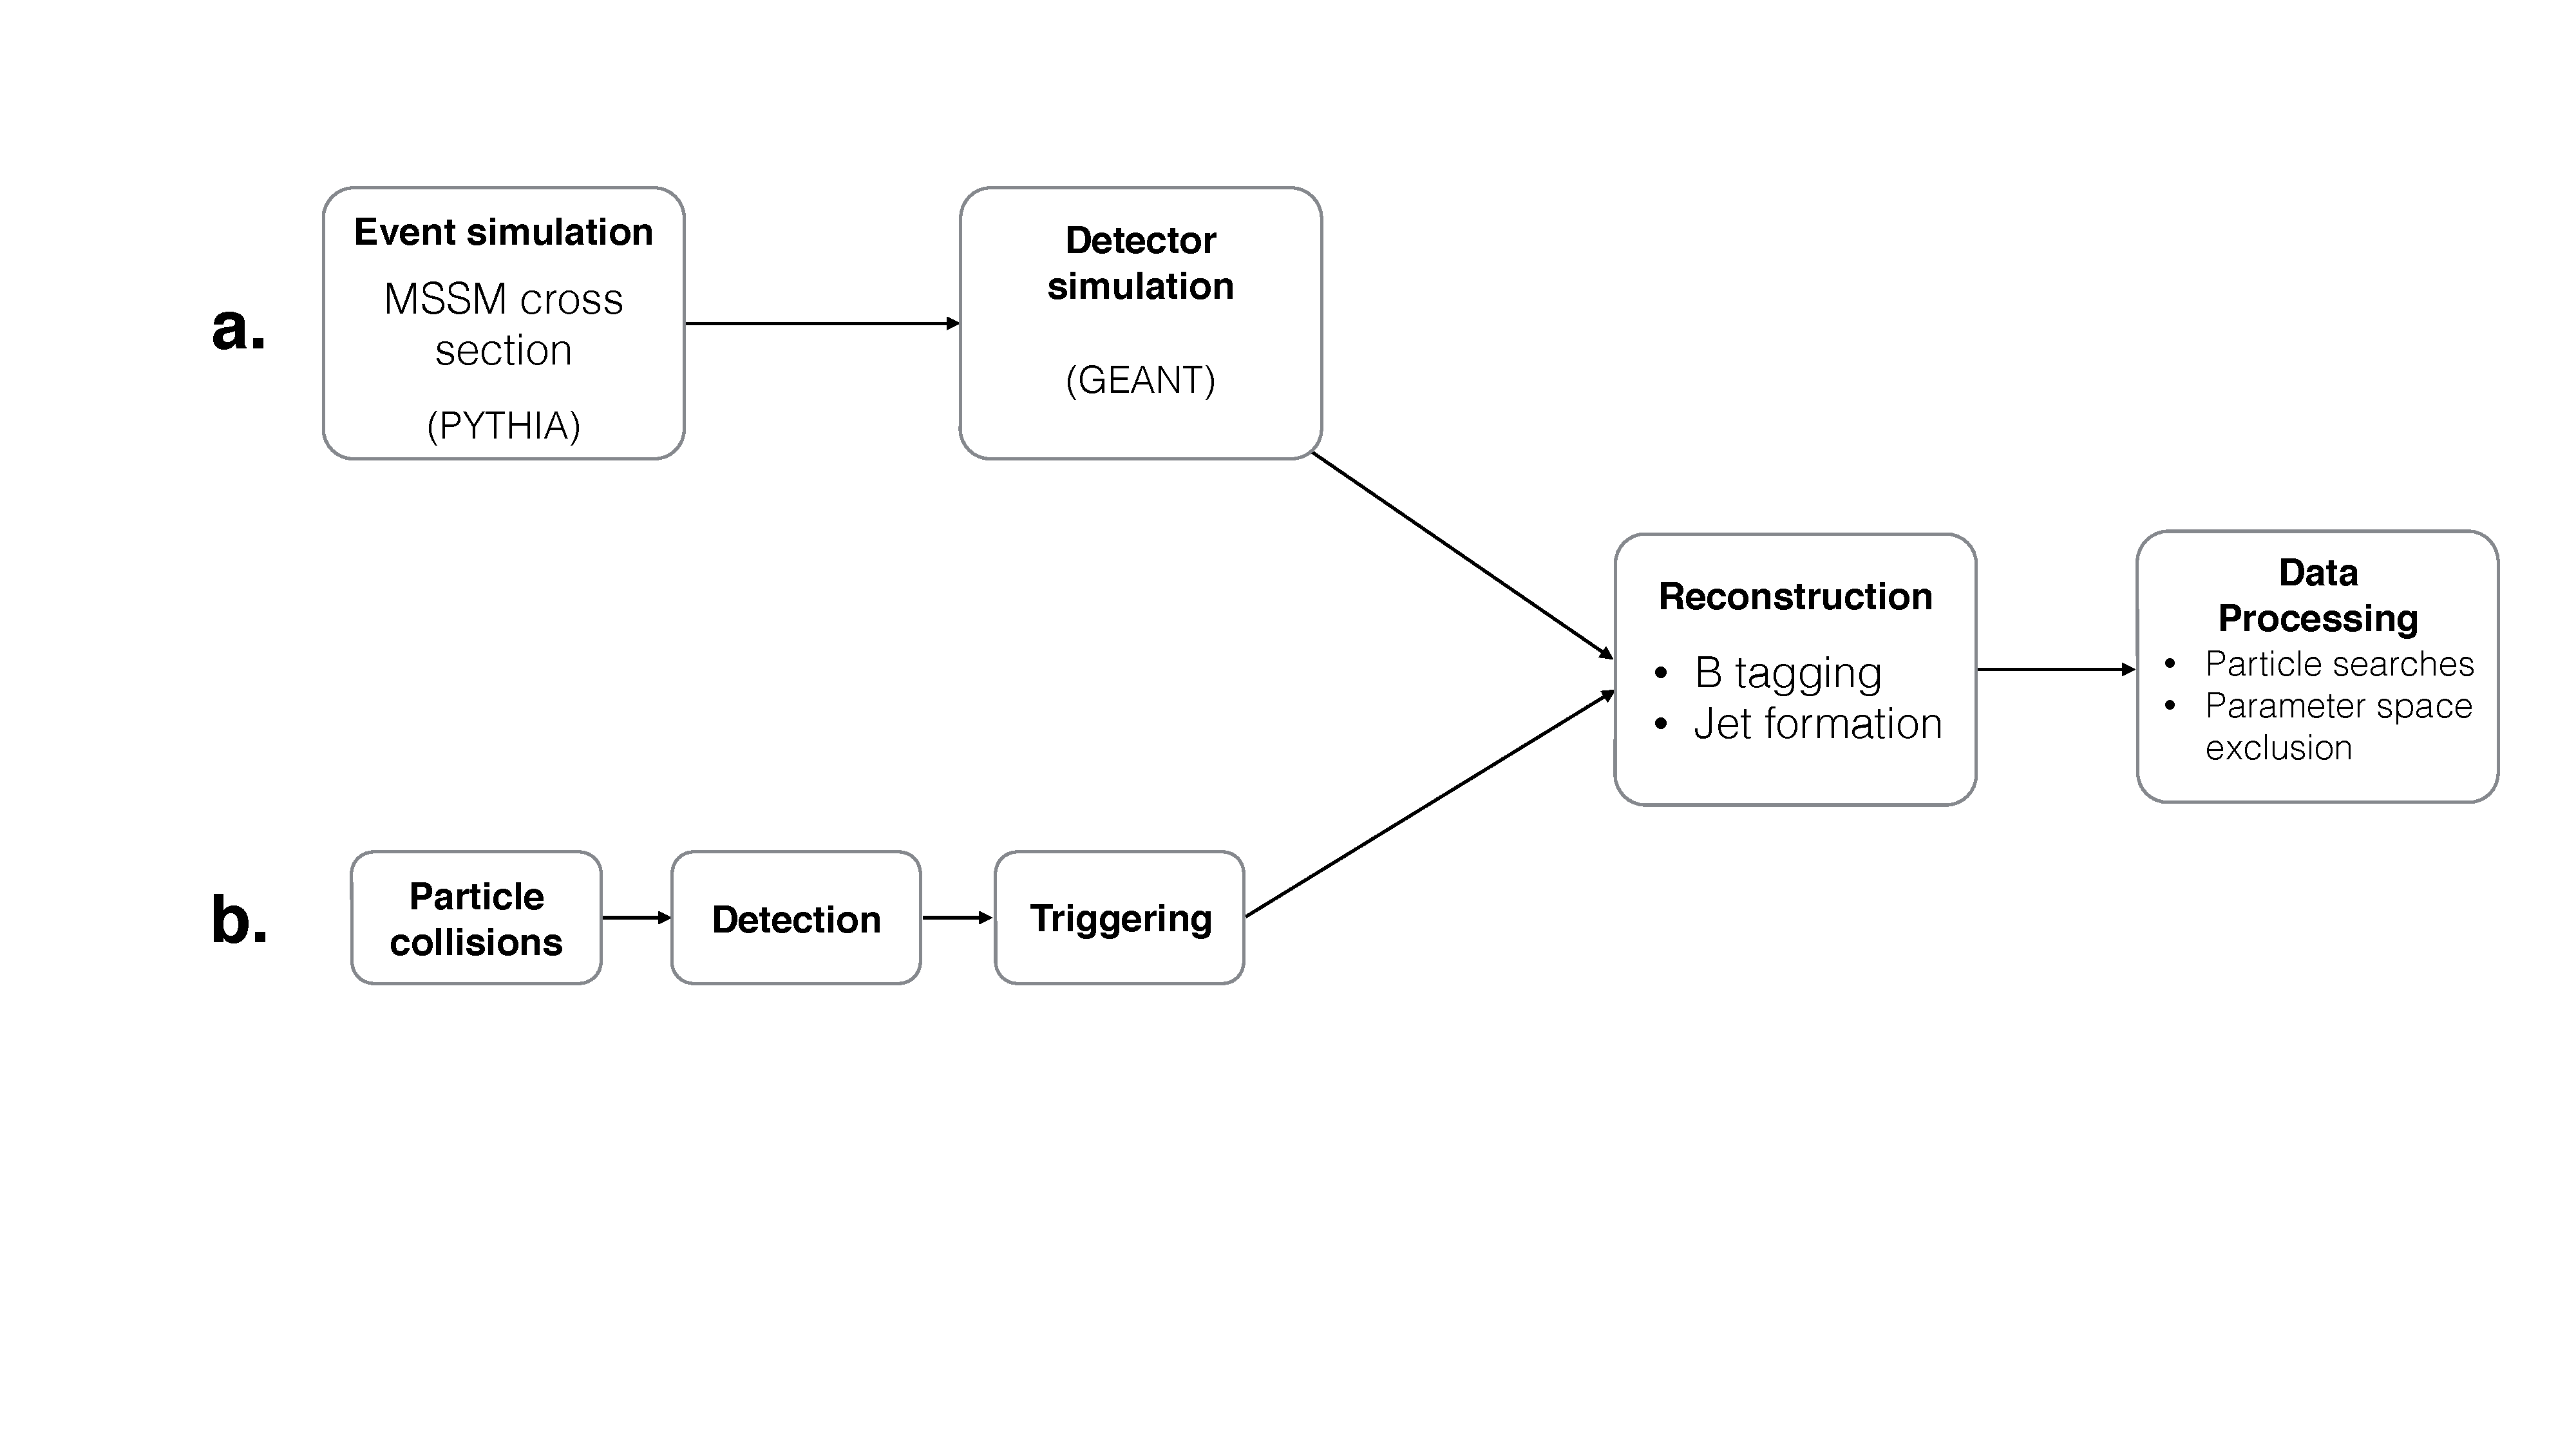
\includegraphics[width=\textwidth]{img/flow}
	\caption{Steps in the information processing pipeline for a. simulated and b. measured data.  }
	\label{fig:flow}
\end{figure}